%TD -- Kapitel 4.1 -- alle Labels darauf aufbauend

%\section{Allgemeines}\label{sec:5.1}
%Um die Charakteristika eines Lautsprechers zu beurteilen ist es wichtig den genauen Frequenzgang eines Lautsprecherchassis zu wissen. Dieser sagt aus, wie sich ein Lautsprecher bei bestimmten Frequenzen verhält. Der von uns gemessene Frequenzbereich beginnt bei 20Hz und endet bei 20kHz. Dieser Bereich wurde gewählt, da auch das menschliche Gehör nur in diesen Frequenzen aktiv ist.
%\begin{figure} [H]
%	\centering
%	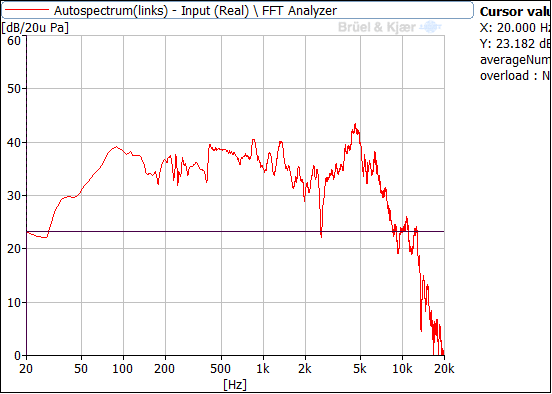
\includegraphics[width=1\textwidth]{img/LSMessung/TT1_9,17l_bestes.png}
%	\caption{Beispiel eines Frequenzganges (Tieftöner PSS 297 58206)}
%	\label{fig:5.1.1}
%\end{figure}
%Anhand dieses Beispiels kann man bereits sehr gut erkennen, wie sich der Schalldruckpegel (hier in dB angegeben) in Abhängigkeit der Frequenz verändert.\newpage
%Da der gemessene Lautsprecher in diesem Fall ein Tieftöner ist, sinkt der Pegel ab einer gewissen Frequenz sehr stark ab. Das bedeutet, dass diese Frequenzen wenig oder gar nicht von dem Lautsprecher abgestrahlt werden - also nicht hörbar sind.\\
%Die Qualität des Frequenzganges eines Lautsprechers hängt nun nicht direkt von dem absoluten Schalldruckpegel ab, sondern viel mehr von den relativen Schwankungen. Der absolute Pegel wird nämlich vom Signal des Verstärkers - im weiteren Sinne vom Benutzer - festgelegt. Das Wichtige dabei ist, was der Lautsprecher aus diesem Signal macht und so entsteht ein Frequenzgang.\\
%In diesem Fall werden hohe Frequenzen vom Lautsprecher \enquote{gedämpft} und somit nicht abgestrahlt.
%
%\subsection{Andere wichtige Eigenschaften eines Lautsprechers}\label{subsec:5.1.1}
%Ein Lautsprecher wird aber nicht nur durch seinen Frequenzgang definiert. Es gibt viele andere Eigenschaften, die auch unter dem Namen \enquote{Thiele-Small-Parameter}\footnote{https://de.wikipedia.org/wiki/Thiele-Small-Parameter,\\Zugriff: 11.02.2017} bekannt sind:
%% Quelle: https://de.wikipedia.org/wiki/Thiele-Small-Parameter
%\begin{itemize}
%	\item Äquivalentvolumen $ V_{as} $
%	\item Resonanzfrequenz $ F_{ms} $
%	\item Elektrische Güte $ Q_{es} $
%	\item Mechanische Güte $ Q_{ms} $
%	\item Gesamtgüte $ Q_{ts} $
%	\item Bewegte Masse $ M_{ms} $
%	\item Membranfläche $ S_{d} $
%	\item Nachgiebigkeit der Aufhängung $ C_{ms} $
%	\item Gleichstromwiderstand $ R_{e} $
%	\item Induktivität der Schwingspule $ L_{e} $
%	\item Verschiebevolumen $ V_{d} $
%	\item maximale Auslenkung $ X_{max} $
%	\item Kraftfaktor \emph{B × l}
%	\item mechanischer Verlustwiderstand $ R_{ms} $
%\end{itemize}
%Diese Eigenschaften, sowie auch die Impedanz \emph{Z}, beschreiben ebenfalls das Verhalten eines Lautsprechers. Sie wurden aber nicht von uns gemessen, weil der Fokus unseres Projekts eher an der Optimierung des Frequenzganges liegt. Die Thiele-Small-Paramter sind außerdem nicht veränderbar, also auch nicht optimierbar.

Um Lautsprecher mit geeigneten Eigenschaften auswählen zu können, müssen zunächst verschiedene Lautsprecher gemessen und verglichen werden.

\section{Messaufbau und Messung}\label{sec:4.1}
Um überhaupt präzise Messungen an Lautsprechern durchführen zu können, benötigt man einen geeigneten Messraum.
Die HTBLuVA St. Pölten verfügt glücklicherweise über so einen reflexionsarmen Raum (Abb. \ref{fig:4.1.1}).
Dieser ist innen mit schalldämpfendem Material ausgekleidet und dämpft somit jede Schallwelle.
Die Anordnung und Struktur der an der Wand befestigten Absorberkeile ist ausschlaggeben dafür, dass der Raum eine möglichst reflexionsfreie Umgebung aufweist.
Der Raum ist auf allen Seiten mit Absorberkeilen bestückt.
Es ist absichtlich ein 6-eckiger Raum um mögliche stehende Wellen noch besser zu unterdrücken.\\
Da es sich nicht um einen schalldichten Raum handelt ist es möglich, dass äußere Einflüsse (Trittschall, Erdbeben,...) das Messergebnis beeinflussen können.
Aus diesem Grund wurden die Messungen bei Verdacht eines äußeren Einflusses erneut gemacht.

\newpage
\begin{figure} [H]
	\centering
	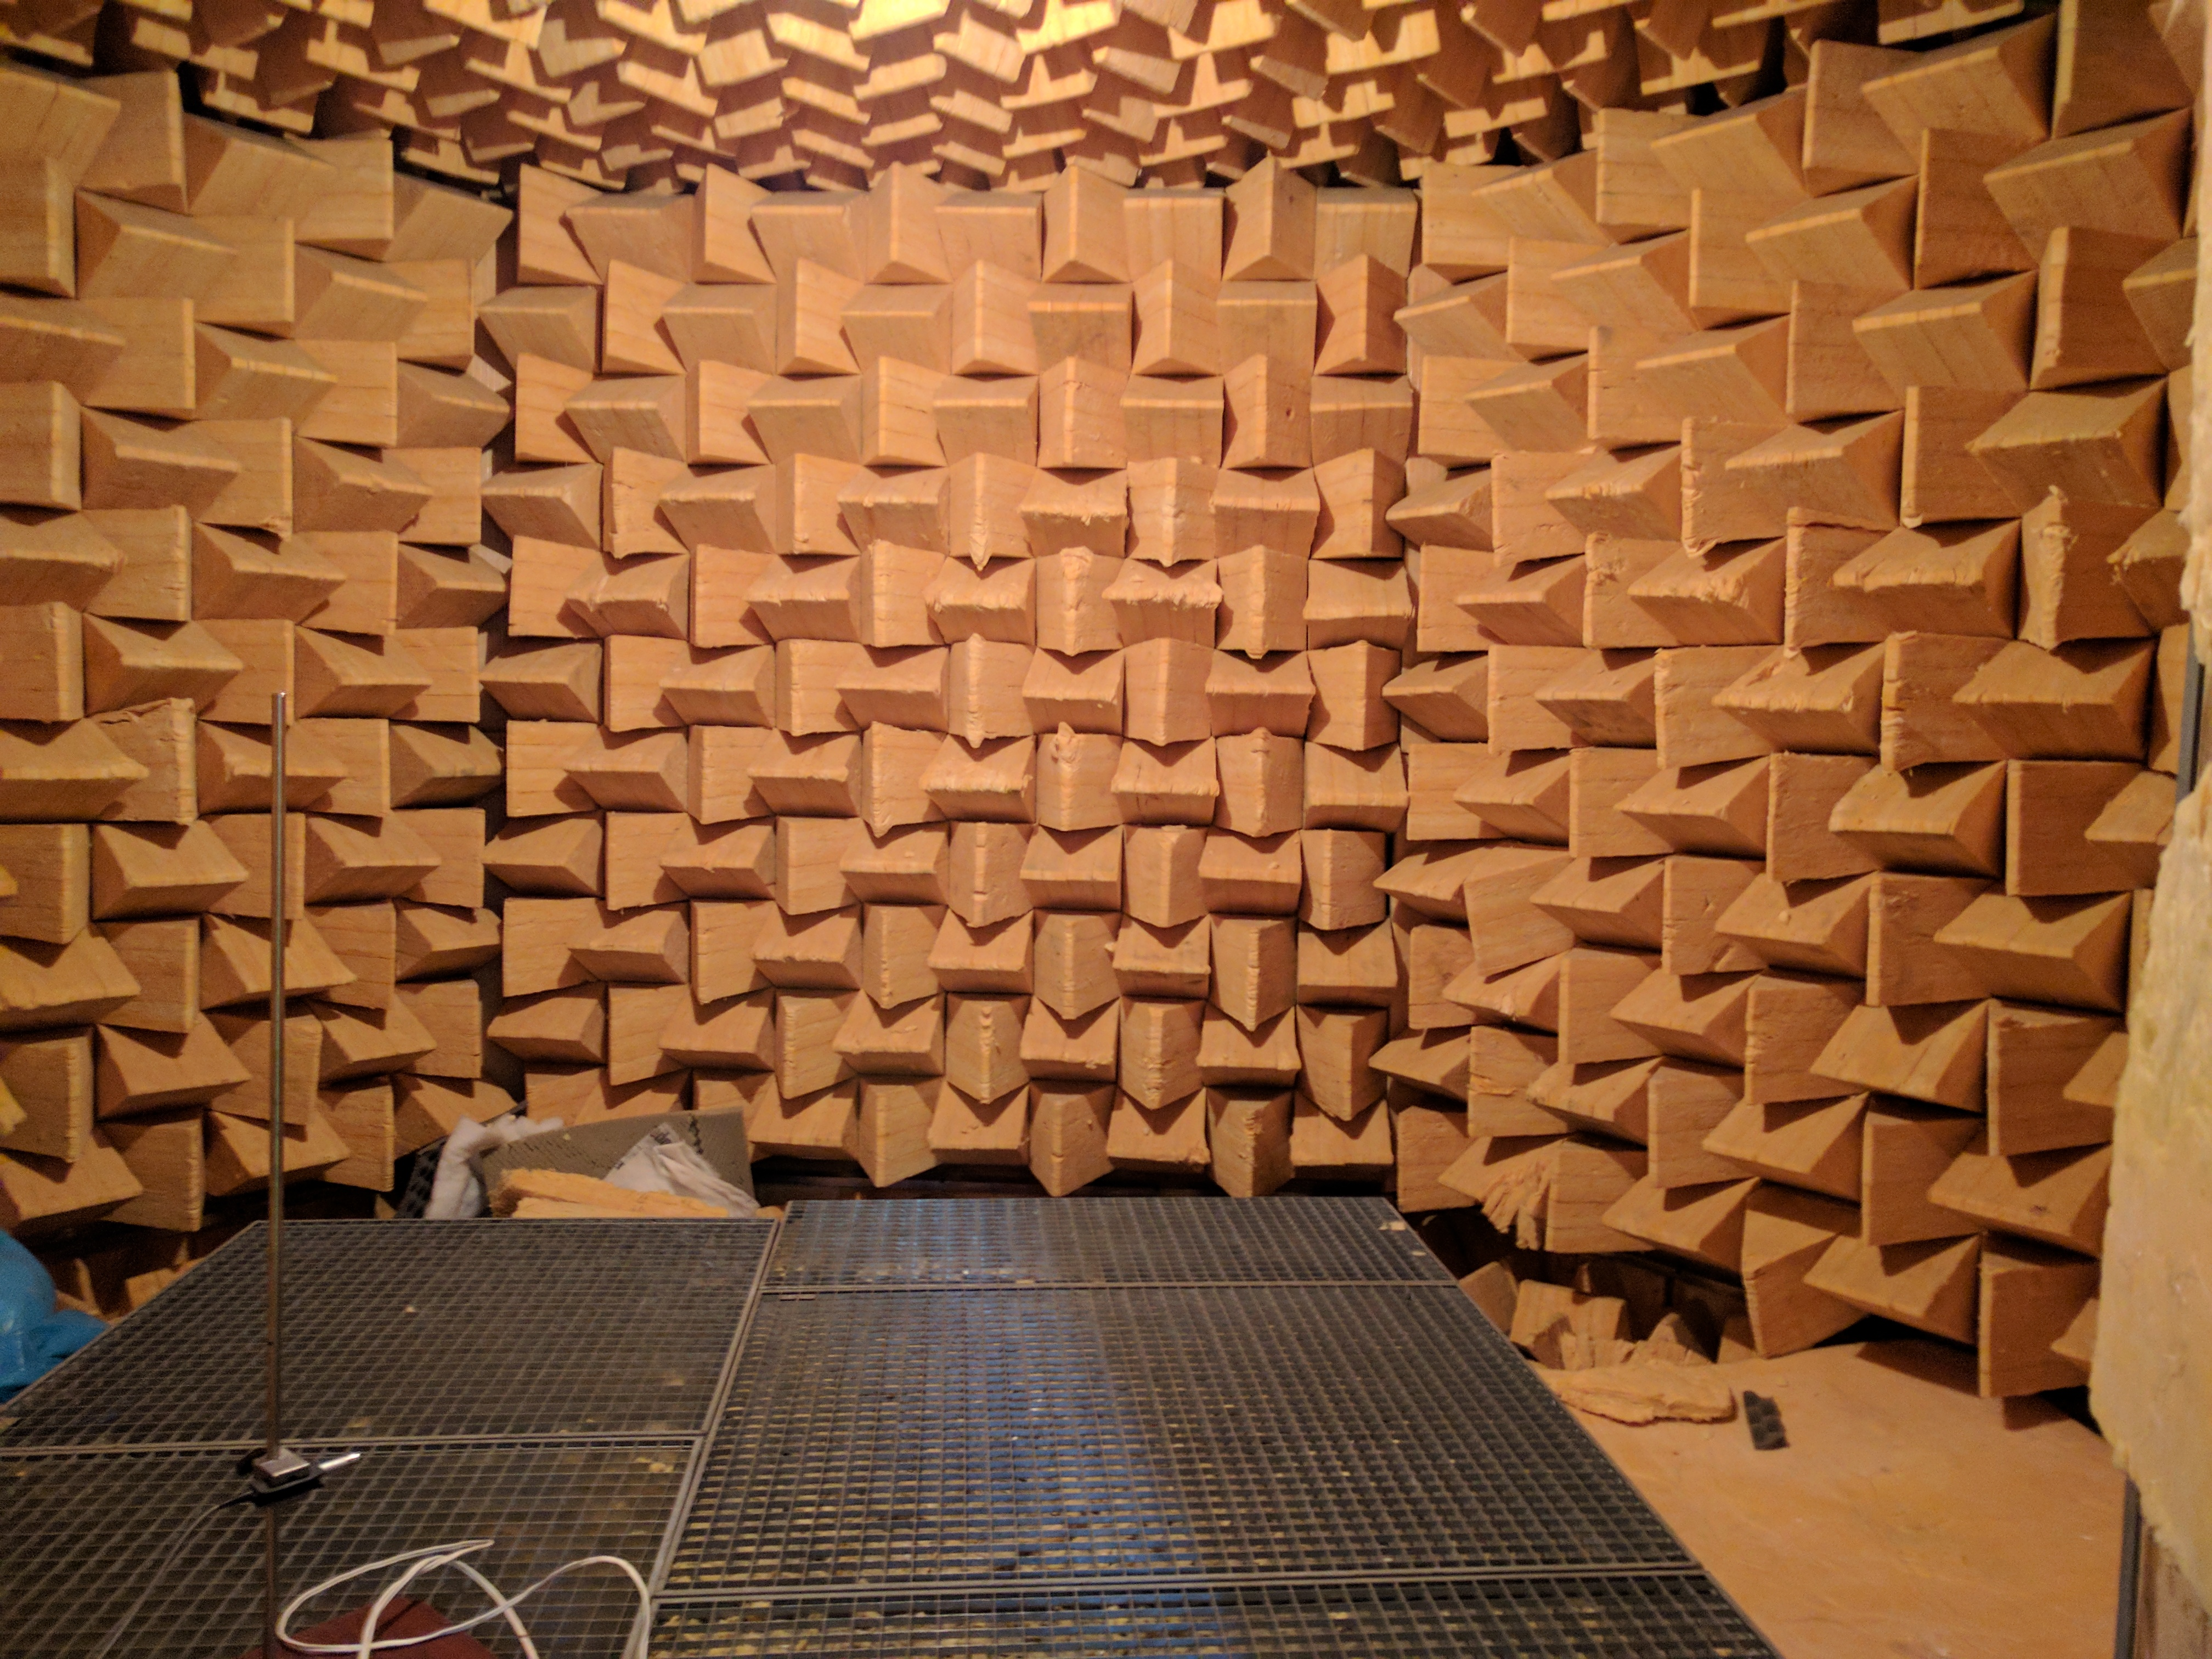
\includegraphics[width=1\textwidth]{img/LSMessung/akkustiklabor1.png}
	\caption{Reflexionsarmer Raum in der HTBLuVA St. Pölten}
	\label{fig:4.1.1}
\end{figure}
%\newpage
In diesem Raum (Abb. \ref{fig:4.1.1}) wurden alle Lautsprecher-Chassis gemessen.\\
Um auch ein passendes Mess-Signal zu erzeugen, ist noch weiteres Equipment nötig:
\begin{itemize}
	\item Mess-Software \enquote{PULSE LabShop Version 13.5.0} von \enquote{Brüel \& Kj\ae r}
	\item USB-Dongle zur Aktivierung der Software
	\item Kalibriertes Messmodul von \enquote{Brüel \& Kj\ae r}
	\item Kalibrierter Signal-Verstärker
	\item Kalibriertes Messmikrofon
	\item Optional: Oszilloskop
	\item Optional: Einstellbares Filter als Frequenzweiche
\end{itemize}

\newpage
\subsection*{Software}\label{subsec:4.1.1}
Als Software wurde \enquote{PULSE LabShop Version 13.5.0} von \enquote{Brüel \& Kj\ae r} verwendet.
Der Mess-PC basiert auf dem Betriebssystem \enquote{Windows XP}.
Um diese Software ordnungsgemäß verwenden zu können, wird noch ein USB-Dongle benötigt.
Nur mit diesem Dongle lässt sich die Software, und somit die Messung, aktivieren.
\begin{figure} [H]
	\centering
	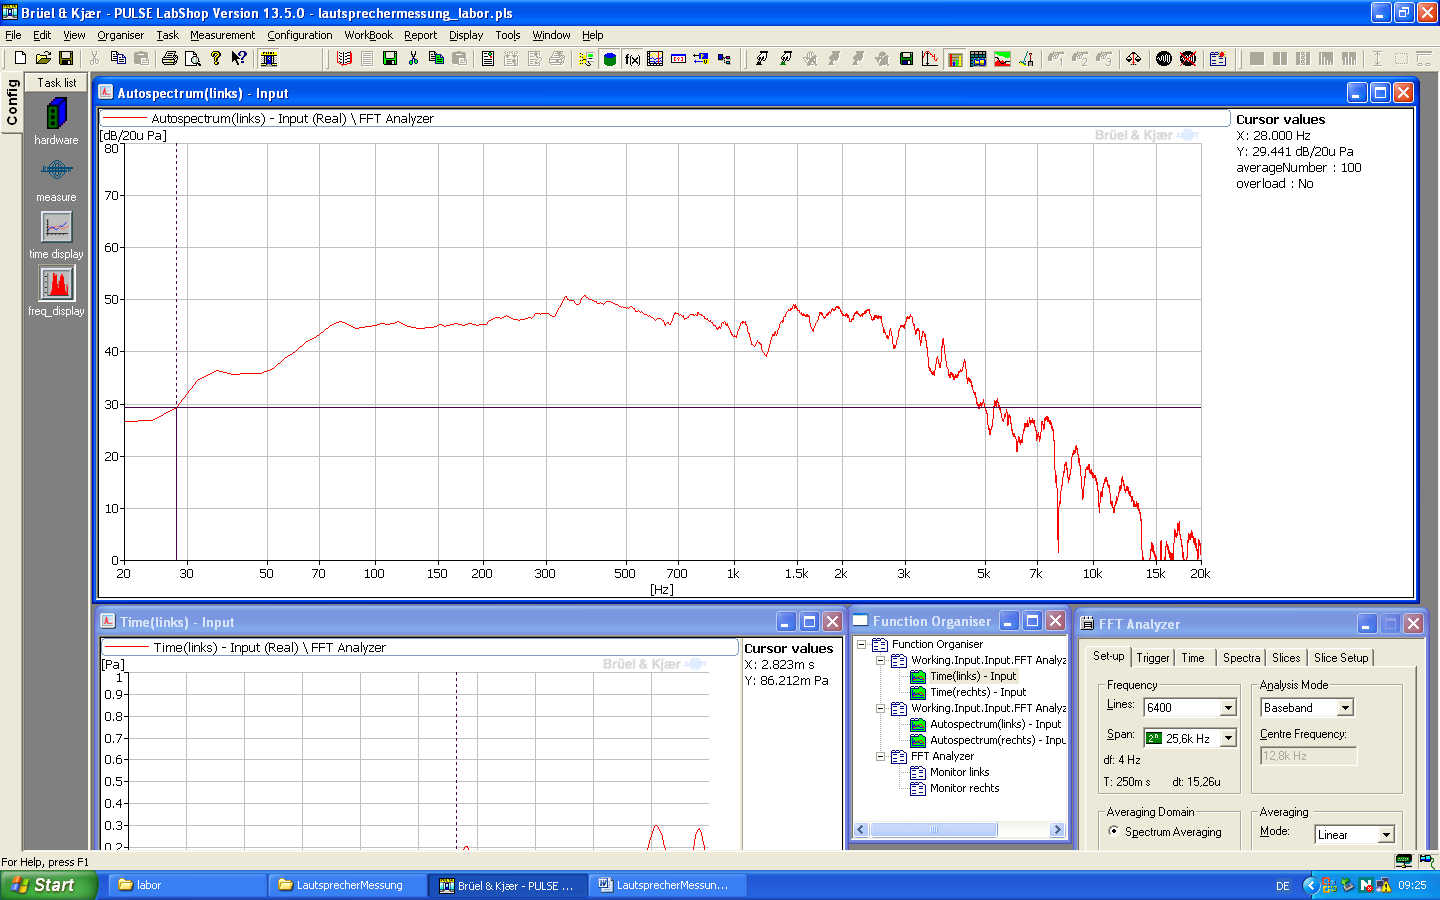
\includegraphics[width=0.8\textwidth]{img/LSMessung/VisatonMitSilikonMitWolle.png}
	\caption{Auschnitt aus der Software \enquote{PULSE LabShop}}
	\label{fig:4.1.1.1}
\end{figure}
In der Abbildung \ref{fig:4.1.1.1} ist bereits ein gemessener Frequenzgang eines Tiefton-Lautsprechers zu sehen.
Bei den Messungen wurde eine abgespeicherte vorkonfigurierte Datei verwendet, damit man nicht immer wieder die nötigen Einstellungen treffen muss.
Die Software ist damit auf alle verwendeten Komponenten abgestimmt und sendet auch das richtige Mess-Signal, ein (\enquote{Weißes Rauschen}), aus.
Mit einem Klick auf die Start-Taste beginnt der Messvorgang.
Es werden insgesamt 100 Messungen gemittelt, um einen möglichst genauen Frequenzgang aufnehmen zu können.
Dies dauert in etwa 20 s.
\\
Die Messeinstellungen sind je nach Wunsch veränderbar, ebenso, wie die Angaben und Einheiten der 2 Achsen.
Die Frequenzachse ist logarithmisch von 20 Hz bis 20 kHz dargestellt.
Die Achse des Schalldruckpegels ist in der logarithmischen Einheit dB (vollständig dBSPL - Sound Pressure Level) angegeben, da die Einheit für Schalldruck \enquote{Pascal} einen Bereich von µPa bis Pa darstellen muss.
Das dB-Maß erleichtert die Veranschaulichung und macht die Kurve übersichtlicher.
In diesem Beispiel (Abb. \ref{fig:4.1.1.1}) ist der Bereich von 0 dB bis 80 dB gewählt.
Diese Einstellung wurde von uns geändert auf 0 dB bis 60 dB, um möglichst vergleichbare Messungen zu erzeugen.\\
Eine logarithmische Frequenzachse und eine Pegelachse von 0 bis 60 (in dB), wird normalerweise für den Vergleich von Lautsprecher-Chassis verwendet.

\newpage
\subsection*{Messmodul}\label{subsec:4.1.2}
Das Messmodul ist über ein Ethernet-Kabel mit dem PC und somit mit der Software verbunden.
Sobald der Befehl zum Start der Messung kommt, beginnt das Modul das Mess-Signal auszusenden und gleichzeitig über das angeschlossene Mikrofon die Ergebnisse aufzunehmen und daraufhin auszuwerten.
\\
Das Mess-Signal besteht aus einem \enquote{weißen Rauschen}.
Dieses Signal ist optimal für die Messung von Lautsprecher-Chassis, da alle Frequenzen mit gleichem Pegel ausgesendet werden.
% Quelle: https://upload.wikimedia.org/wikipedia/commons/c/c1/White_noise.svg
% Quelle: https://upload.wikimedia.org/wikipedia/commons/3/3c/White_noise_spectrum.svg
\begin{figure} [H]
	\centering
	\subfloat{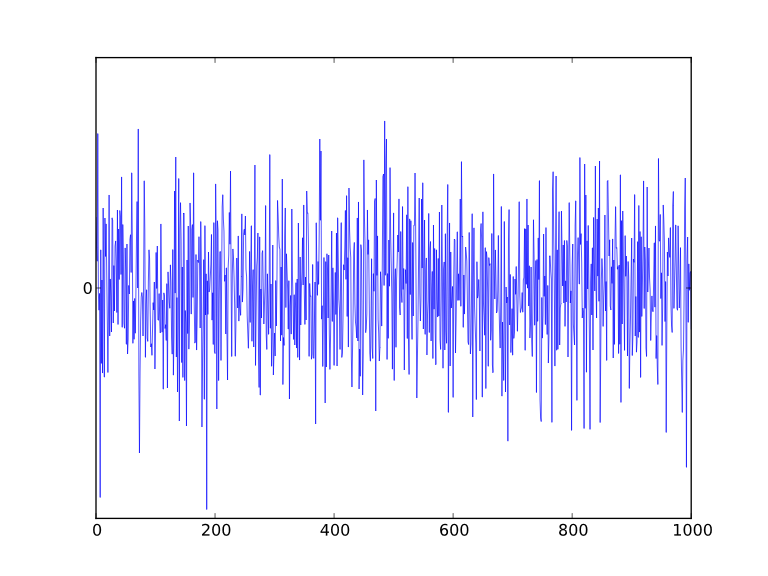
\includegraphics[valign=m,width=0.4\textwidth]{img/LSMessung/White_noise.png}}
	\subfloat{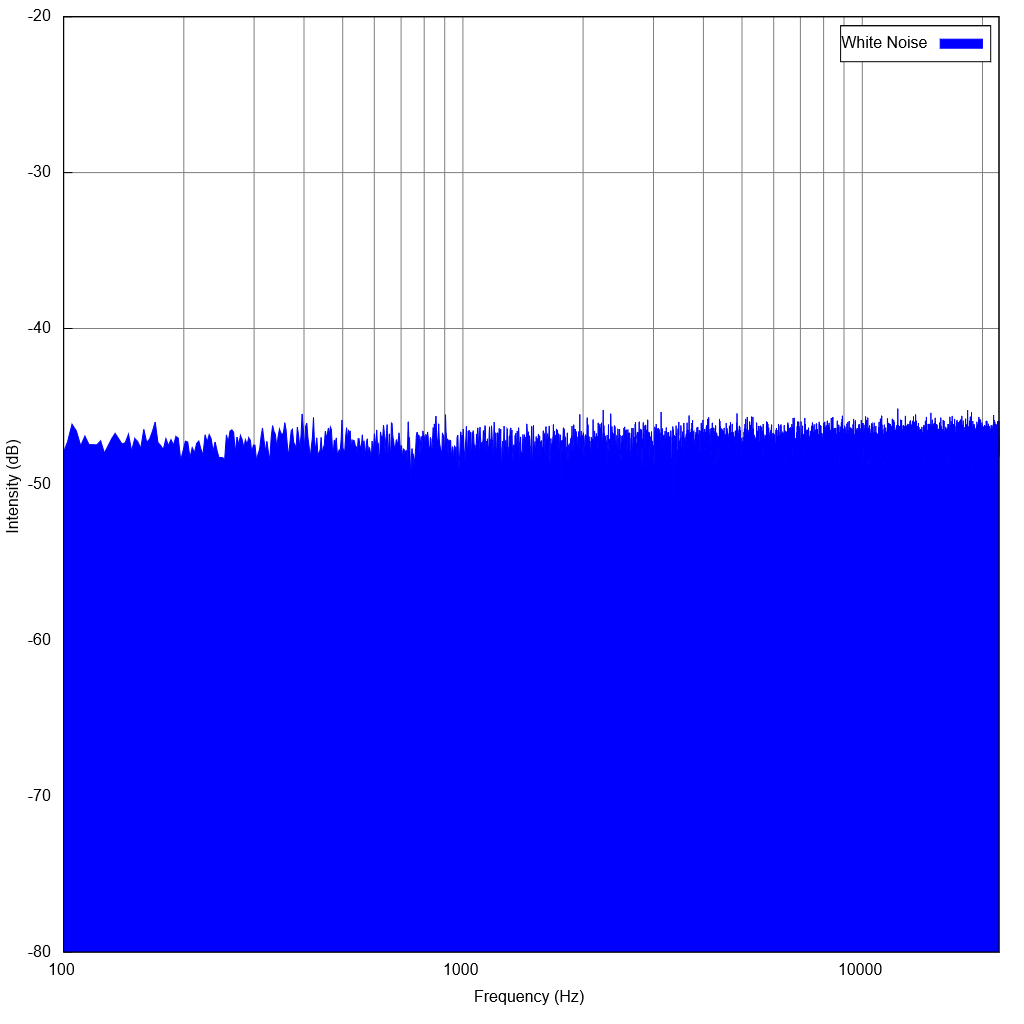
\includegraphics[valign=m,width=0.4\textwidth]{img/LSMessung/White_noise_spectrum.png}}
	\caption[Zeitfunktion und Spektrum von \enquote{weißem Rauschen}]{Zeitfunktion\footnotemark und Spektrum\footnotemark von \enquote{weißem Rauschen}}
	\label{fig:4.1.2.1}
\end{figure}
\footnotetext[1]{https://upload.wikimedia.org/wikipedia/commons/c/c1/White\_noise.svg,\\Zugriff: 11.02.2017}
\footnotetext[2]{https://upload.wikimedia.org/wikipedia/commons/3/3c/White\_noise\_spectrum.svg,\\Zugriff: 11.02.2017}
\begin{figure} [H]
	\centering
	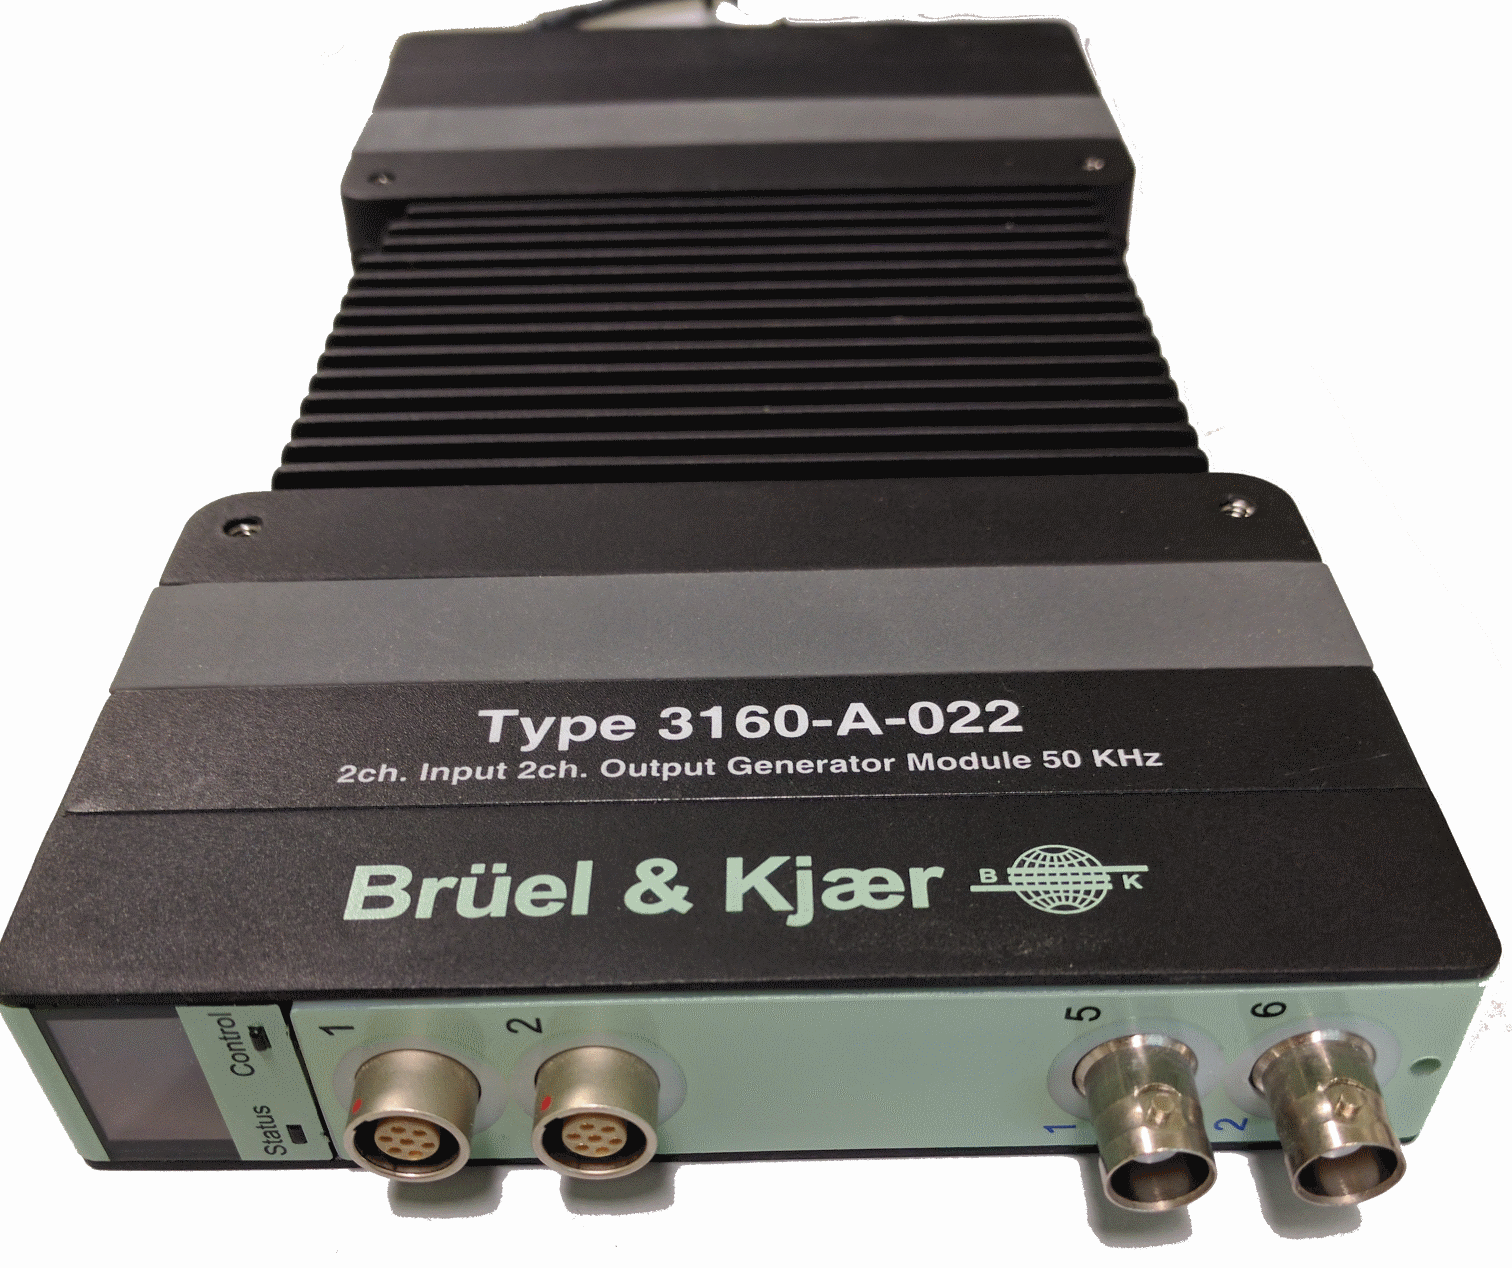
\includegraphics[width=0.4\textwidth]{img/LSMessung/modul_front.png}
	\caption{Messmodul}
	\label{fig:4.1.2.2}
\end{figure}

\newpage
\subsection*{Verstärker}\label{subsec:4.1.3}
Prinzipiell kann für diesen Aufbau jeder Leistungsverstärker verwendet werden.
In unserem Fall war ein kalibrierter \enquote{Brüel \& Kj\ae r Power Amplifier Type 2706} in Verwendung.
\\
Da meist nur ein Lautsprecher gemessen wird, benötigt man auch nur ein Signal (Mono, kein Stereo) zum Messen.
Der Verstärker verfügt über einen in Stufen schaltbaren Abschwächer und einen stufenlosen \enquote{Gain Control}.\\
Da die anderen Messkomponenten in dem Aufbau auch von der Firma  \enquote{Brüel \& Kj\ae r} sind, weist der Verstärker eine hohe Kompatibilität zum restlichen Equipment auf.
\begin{figure} [H]
	\centering
	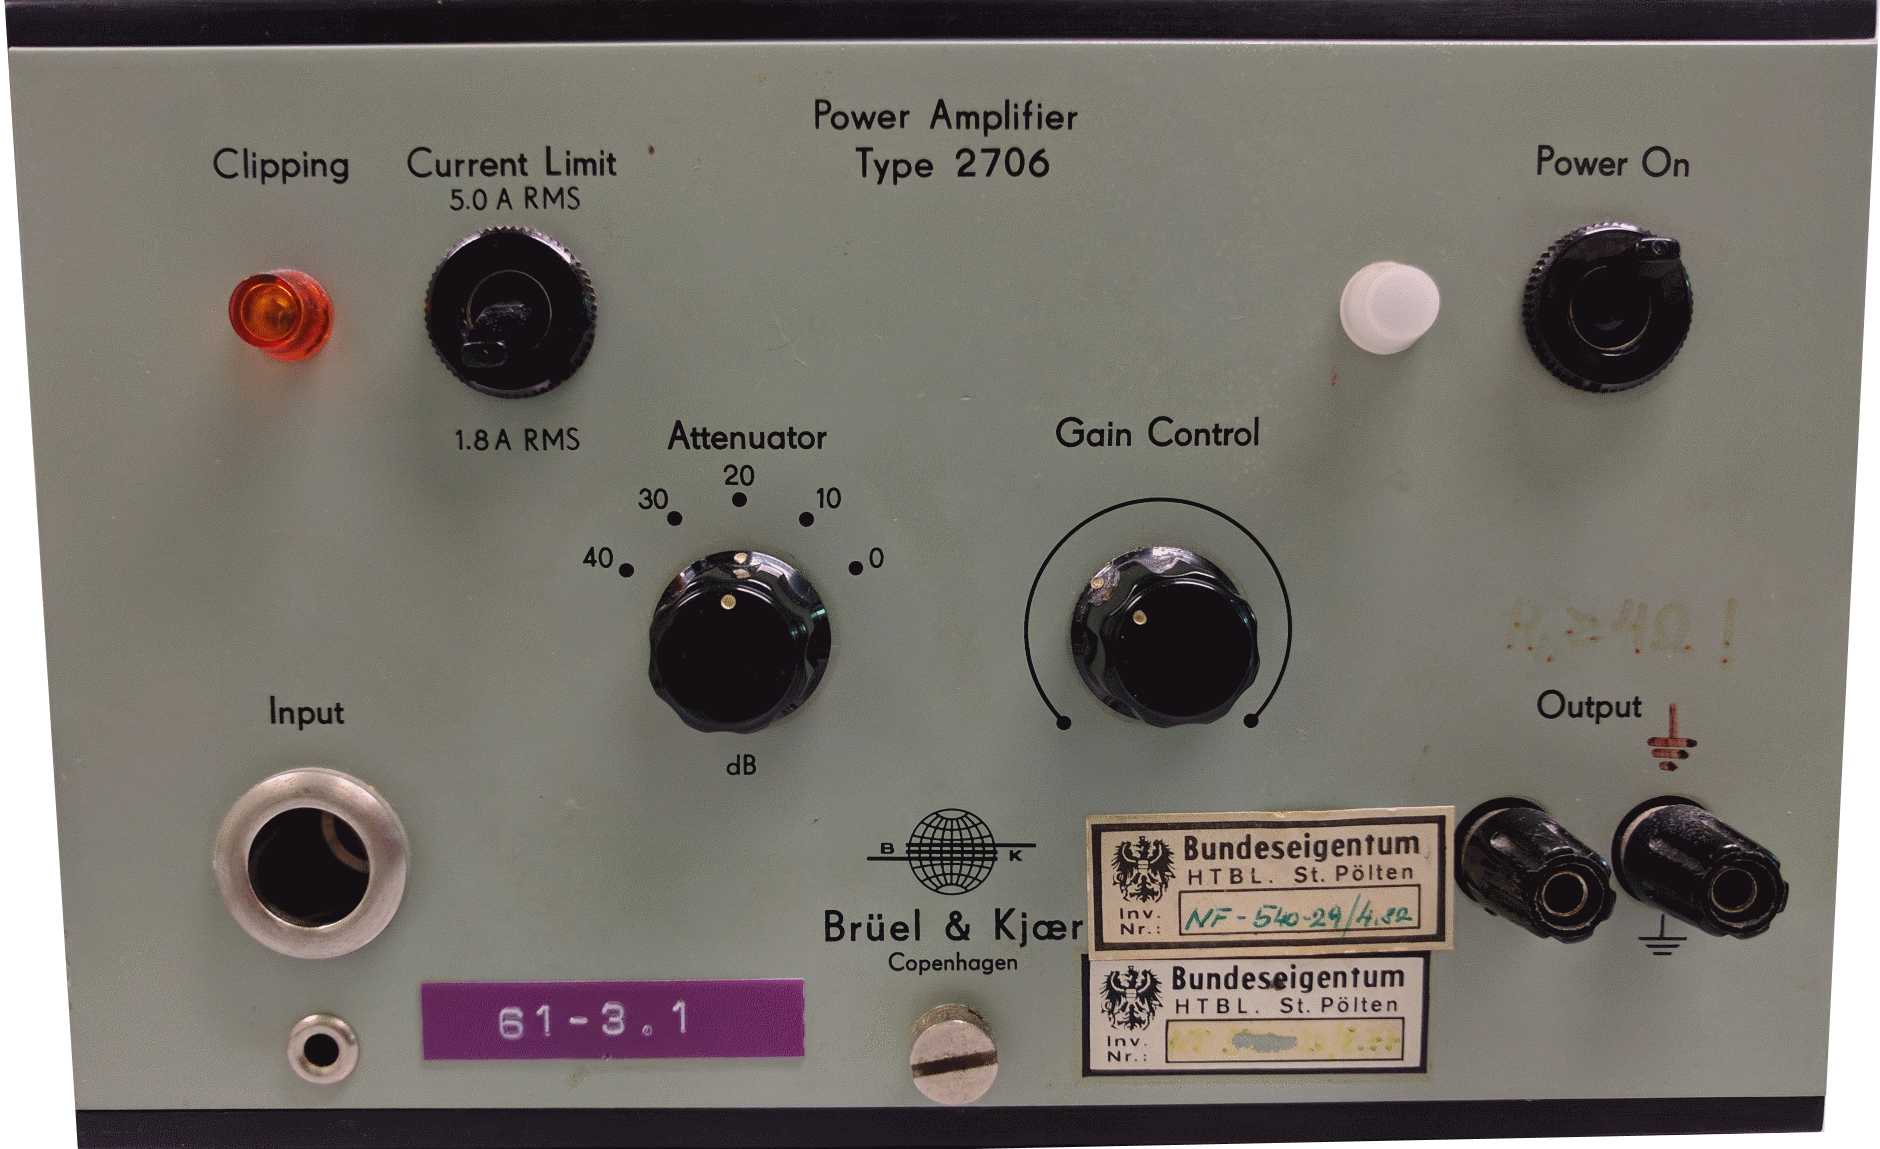
\includegraphics[width=0.4\textwidth]{img/LSMessung/verstaerker1V2.png}
	\caption{\enquote{Brüel \& Kj\ae r Power Amplifier Type 2706}}
	\label{fig:4.1.3.1}
\end{figure}

\subsection*{Messmikrofon}\label{subsec:4.1.4}
Um den Schalldruckpegel möglichst präzise messen zu können, wird auch ein dementsprechend genaues und kalibriertes Messmikrofon benötigt.
In diesem Projekt wurde das Messmikrofon \enquote{Brüel \& Kj\ae r Type 2669} verwendet.
\\
Ebenfalls wichtig ist die Ausrichtung des Messmikrofons.
Es sollte immer auf den Lautsprecher zentriert (horizontal und vertikal) angebracht werden.
Die Entfernung zum Messobjekt (1 m) muss bei verschiedenen Lautsprechern gleich bleiben, um vergleichbare Messungen zu ermöglichen.
Bei einem Zwei-Weg-System (Hoch- und Tiefton-Lautsprecher) wurde das Mikrofon (vertikal gesehen) zwischen den Lautsprechern befestigt.
\begin{figure} [H]
	\centering
	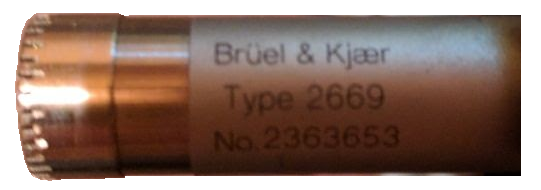
\includegraphics[width=0.4\textwidth]{img/LSMessung/mikroV2.png}
	\caption{Messmikrofon \enquote{Brüel \& Kj\ae r Type 2669}}
	\label{fig:4.1.4.1}
\end{figure}